% Тип документа
\documentclass[a4paper,12pt]{extarticle}

% Шрифты, кодировки, символьные таблицы, переносы
\usepackage{cmap}
\usepackage[T2A]{fontenc}
\usepackage[utf8x]{inputenc}
\usepackage[russian]{babel}

% Это пакет -- хитрый пакет, он нужен но не нужен
\usepackage[mode=buildnew]{standalone}

\usepackage
	{
		% Дополнения Американского математического общества (AMS)
		amssymb,
		amsfonts,
		amsmath,
		amsthm,
		physics,
		% misccorr,
		% Шрифт для буковок  
		dsfont,
		% Графики и рисунки
		wrapfig,
		graphicx,
		subcaption,
		float,
		tikz,
		tikz-3dplot,
		caption,
		csvsimple,
		color,
		booktabs,
		pgfplots,
		pgfplotstable,
		geometry,
		% 
		% Таблицы, списки
		array,
		makecell,
		multirow,
		indentfirst,
		%
		% Интегралы и прочие обозначения
		ulem,
		esint,
		esdiff,
		% 
		% Колонтитулы
		fancyhdr,
	}  

\usepackage{xcolor}
\usepackage{hyperref}

 % Цвета для гиперссылок
\definecolor{linkcolor}{HTML}{000000} % цвет ссылок
\definecolor{urlcolor}{HTML}{799B03} % цвет гиперссылок
 
\hypersetup{pdfstartview=FitH,  linkcolor=linkcolor,urlcolor=urlcolor, colorlinks=true}
% Обводка текста в TikZ
\usepackage[outline]{contour}

% Увеличенный межстрочный интервал, французские пробелы
\linespread{1.3} 
\frenchspacing 

 
\usetikzlibrary
	{
		decorations.pathreplacing,
		decorations.pathmorphing,
		patterns,
		calc,
		scopes,
		arrows,
		fadings,
		through,
		shapes.misc,
		arrows.meta,
		3d,
		quotes,
		angles,
		babel
	}


\tikzset{
	force/.style=	{
		>=latex,
		draw=blue,
		fill=blue,
				 	}, 
	%				 	
	axis/.style=	{
		densely dashed,
		blue,
		line width=1pt,
		font=\small,
					},
	%
	th/.style=	{
		line width=1pt},
	%
	acceleration/.style={
		>=open triangle 60,
		draw=magenta,
		fill=magenta,
					},
	%
	inforce/.style=	{
		force,
		double equal sign distance=2pt,
					},
	%
	interface/.style={
		pattern = north east lines, 
		draw    = none, 
		pattern color=gray!60,
					},
	cross/.style=	{
		cross out, 
		draw=black, 
		minimum size=2*(#1-\pgflinewidth), 
		inner sep=0pt, outer sep=0pt,
					},
	%
	cargo/.style=	{
		rectangle, 
		fill=black!70, 
		inner sep=2.5mm,
					},
	%
	caption/.style= {
		midway,
		fill=white!20, 
		opacity=0.9
					},
	%
	}

\newenvironment{tikzpict}
    {
	    \begin{figure}[htbp]
		\centering
		\begin{tikzpicture}
    }
    { 
		\end{tikzpicture}
		% \caption{caption}
		% \label{fig:label}
		\end{figure}
    }


\tikzset{
	coordsys/.style={scale=1.8,x={(1.1cm,-0cm)},y={(0.5cm,1cm)}, z={(0cm,0.8cm)}},
	coordsys/.style={scale=1.5,x={(0cm,0cm)},y={(1cm,0cm)}, z={(0cm,1cm)}}, 
	coordsys/.style={scale=1.5,x={(1cm,0cm)},y={(0cm,1cm)}, z={(0cm,0cm)}}, 
}

\usepgfplotslibrary{units}

% Среднее <#1>
\newcommand{\mean}[1]{\langle#1\rangle}

\pgfplotsset{
    % most recent feature set of pgfplots
    compat=newest,
}

% const прямым шрифтом
\newcommand\ct[1]{\text{\rmfamily\upshape #1}}
\newcommand*{\const}{\ct{const}}


\usepackage[europeanresistors,americaninductors]{circuitikz}

% Style to select only points from #1 to #2 (inclusive)
\pgfplotsset{select/.style 2 args={
    x filter/.code={
        \ifnum\coordindex<#1\def\pgfmathresult{}\fi
        \ifnum\coordindex>#2\def\pgfmathresult{}\fi
    }
}}


\usepackage{array}
\usepackage{pstool}


%%%%%%%%%%%%%%%%%%%%%%%%%%%%%%%%%%%%%%%%%%%%%%%%%
\makeatletter
\newif\if@gather@prefix 
\preto\place@tag@gather{% 
  \if@gather@prefix\iftagsleft@ 
    \kern-\gdisplaywidth@ 
    \rlap{\gather@prefix}% 
    \kern\gdisplaywidth@ 
  \fi\fi 
} 
\appto\place@tag@gather{% 
  \if@gather@prefix\iftagsleft@\else 
    \kern-\displaywidth 
    \rlap{\gather@prefix}% 
    \kern\displaywidth 
  \fi\fi 
  \global\@gather@prefixfalse 
} 
\preto\place@tag{% 
  \if@gather@prefix\iftagsleft@ 
    \kern-\gdisplaywidth@ 
    \rlap{\gather@prefix}% 
    \kern\displaywidth@ 
  \fi\fi 
} 
\appto\place@tag{% 
  \if@gather@prefix\iftagsleft@\else 
    \kern-\displaywidth 
    \rlap{\gather@prefix}% 
    \kern\displaywidth 
  \fi\fi 
  \global\@gather@prefixfalse 
} 
\newcommand*{\beforetext}[1]{% 
  \ifmeasuring@\else
  \gdef\gather@prefix{#1}% 
  \global\@gather@prefixtrue 
  \fi
} 
\makeatother
%%%%%%%%%%%%%%%%%%%%%%%%%%%%%%%%%%%%%%%%%%%%%%%%%

\geometry		
	{
		left			=	2cm,
		right 			=	2cm,
		top 			=	3cm,
		bottom 			=	3cm,
		bindingoffset	=	0cm
	}

%%%%%%%%%%%%%%%%%%%%%%%%%%%%%%%%%%%%%%%%%%%%%%%%%%%%%%%%%%%%%%%%%%%%%%%%%%%%%%%



	%применим колонтитул к стилю страницы
\pagestyle{fancy} 
	%очистим "шапку" страницы
\fancyhead{} 
	%слева сверху на четных и справа на нечетных
\fancyhead[R]{\labauthors} 
	%справа сверху на четных и слева на нечетных
\fancyhead[L]{Отчёт по лабораторной работе №\labnumber} 
	%очистим "подвал" страницы
\fancyfoot{} 
	% номер страницы в нижнем колинтуле в центре
\fancyfoot[C]{\thepage} 

%%%%%%%%%%%%%%%%%%%%%%%%%%%%%%%%%%%%%%%%%%%%%%%%%%%%%%%%%%%%%%%%%%%%%%%%%%%%%%%

\renewcommand{\contentsname}{Оглавление}

\usepackage{tocloft}

\renewcommand{\cftsecleader}{\cftdotfill{\cftdotsep}}

\usepackage{secdot}
\sectiondot{subsection}

\begin{document}

\def\labauthors{Виноградов И.Д., Шиков А.П.}
\def\labgroup{430}
\def\labnumber{2}
\def\labtheme{Измерение импедансов и коэффициентов отражения}
\begin{titlepage}

\begin{center}

{\small\textsc{Нижегородский государственный университет имени Н.\,И. Лобачевского}}
\vskip 1pt \hrule \vskip 3pt
{\small\textsc{Радиофизический факультет. Кафедра Электродинамики.}}

\vfill

{\Large Отчет по лабораторной работе №\labnumber\vskip 12pt\bfseries \labtheme}
	
\end{center}

\vfill
	
\begin{flushright}
	{Выполнили студенты \labgroup\ группы\\ \labauthors}%\vskip 12pt Принял:\\ Менсов С.\,Н.}
\end{flushright}
	
\vfill
	
\begin{center}
	Нижний Новгород, \the\year
\end{center}

\end{titlepage}



\newpage

{\bfseries Цель работы:} 
определение импедансов и коэффициентов отражения заданных нагрузок с помощью волноводной измерительной линии.

\section{Теоритическая часть}

Поле в регулярной линии передач может быть представлено в виде суперпозиции собственных волн вида $ \cos (\omega t \pm h
z + \varphi) $, или, в комплексном виде: $e^{ i ( \omega t \pm h z +\varphi ) }$. 

Важной характеристикой собственной волны (моды) является характеристический импеданс $Z_{\bot}$, определяющийся как отношение:
\begin{equation}
     \textbf{E}_{\bot} = Z_{\bot}[ \textbf{H}_{\bot},\textbf{n} ]
    \label{eq:1}
\end{equation}
где \textbf{n} - единичный вектор в направлении распространения волны. В случае бегущей волны без потерь, $Z_{\bot} \in
\mathds{R} $. Для нераспространяющихся волн величина $Z_{\bot} \in \mathds{C} \Rightarrow Z_{\bot} = iZ'$ (В частности
$Z'>0$ для волн $TE$ - типа, и $Z'<0$ для волн $TM$ - типа). 

В ЛП с произвольной нагрузкой на конце поле волны представляет собой суперпозицию прямой и обратной волн:
\begin{equation}
    \begin{split}
        \textbf{E}(\textbf{r}_{\bot},z,t) = \textbf{E}^+(\textbf{r}_{\bot},z,t)+\textbf{E}^-(\textbf{r}_{\bot},z,t),\\
        \textbf{H}(\textbf{r}_{\bot},z,t) = \textbf{H}^+(\textbf{r}_{\bot},z,t)+\textbf{H}^-(\textbf{r}_{\bot},z,t),  
    \end{split}
    \label{eq:2}
\end{equation}
$\textbf{E}^+,\textbf{H}^+$ - распростроняющиеся в положительном направлении, $\textbf{E}^-,\textbf{H}^-$ -
распростроняющиеся в отрицательном направлении.

В волноводах, для кадого типа волны можно разделить зависимость полей от поперечных ($\textbf{r}_{\bot}$) и продольной
($z$) координат и представить поле каждой из волн в виде:
\begin{equation}
    \begin{split}
        \textbf{E}^{\pm}(\textbf{r}_{\bot},z,t) = \mathcal{E} (\textbf{r}_{\bot}) U^{\pm}(z,t),\\
        \textbf{H}^{\pm}(\textbf{r}_{\bot},z,t) = \mathcal{H} (\textbf{r}_{\bot}) I^{\pm}(z,t),  
    \end{split}
    \label{eq:3}
\end{equation}
где $ \mathcal{E}, \mathcal{H}$ - соответствующим образом нормированные векторные функции, описывающие распределение
полей в поперечном сечении волновода. Для скалярных функций имеем:
\begin{equation}
    \begin{split}
        U(z,t) = U^+(z,t)+U^-(z,t),\\
        I(z,t) = I^+(z,t)+I^-(z,t),  
    \end{split}
    \label{eq:4}
\end{equation}
Эти функции в общем случае называют условными напряжением и током. В данной работе будет использоваться коаксиальная
линия передач, поэтому можно вкратце описать получение таких токов и напряжений для оаксиальной линии.
% \begin{center}
%     \begin{figure}[h!]
%         \centering
%         \includegraphics[width = 0.5\linewidth]{example-image-a}
%         \label{fig:1}
%         \caption{Поперечное сечение коаксиальной ЛП}
%     \end{figure}
% \end{center}
В цилиндрической системе коорднат будем иметь компоненты полей: 
\begin{equation}
    E_r = \frac{A}{r} e^{iw(t-\frac{z}{v})},~~ H_{\varphi} = \frac{E_r}{\eta}
    \label{eq:5}
\end{equation}
где $\eta = \sqrt{\mu / \varepsilon}$ - волновой импеданс среды, $v = \frac{c}{\sqrt{\varepsilon \mu}}$ - скорость света в
среде. Напряжение между проводниками, и ток центрального проводника:
\begin{equation}
    U = \int \limits_a^b E_r dr = A ln \frac{b}{a} e^{iw(t-\frac{z}{v})},~~~~
    I_a = \frac{c}{4 \pi } \oint \limits_L H_{\varphi} dl = \frac{A c}{2 \eta} e^{iw(t-\frac{z}{v})}
    \label{eq:6}
\end{equation}

При подстановке в \eqref{eq:3} можем получить вид функций $\mathcal{E},\mathcal{H}$:
\begin{equation}
        \mathcal{E} =\frac{1}{r~ ln~ b/a},~~\mathcal{H} = \frac{2}{c r},  
    \label{eq:8}
\end{equation}
а при подстановке соотношений \eqref{eq:8} в уравнения Максвелла, можно получить телеграфные уравнения:
\begin{equation}
        \frac{L}{c^2} \frac{ \partial I}{\partial t} + \frac{\partial U}{\partial z} = 0,~~
        C \frac{ \partial U}{\partial t} + \frac{\partial I}{\partial z} = 0,
    \label{eq:9}
\end{equation}
$C,L$ -погонная емкость и индуктивность:
\begin{equation}
    C = \frac{\varepsilon}{2 ln ~b/a},~~ L = 2 \mu ~ln~ b/a.
    \label{eq:10}
\end{equation}
При описании мод в токах и напряжениях, удобно ввести волновое сопротивление $Z_B$, в частности для коаксиальной линии :
\begin{equation}
    Z_B = \pm \frac{U^{\pm}}{I^{\pm}} = \frac{1}{c} \sqrt{\frac{L}{C}} = \frac{1}{c} \sqrt{\frac{\mu}{\varepsilon}}~ln (\frac{b}{a})
    \label{eq:11}
\end{equation}

Важная информация о структуре поля содержится в отношениях комплексных амплитуд: имепданс $Z$ и коэффициент отражения
$\Gamma$ в сечении $z$:
\begin{equation}
    Z(z) = \frac{U(z)}{I(z)} = \frac{U^+(z)+U^-(z)}{I^+(z)+I^-(z)},~~ \Gamma(z)=\frac{U^-(z)}{U^+(z)} = \frac{I^-(z)}{I^+(z)}.
    \label{eq:12}
\end{equation}
В каждом сечении величины $\Gamma$ и $Z$ связаны соотношениями:
\begin{equation}
    Z(z) = Z_B\frac{1+\Gamma(z)}{1-\Gamma(z)},~~\Gamma = \frac{Z(z)-Z_B}{Z(z)+Z_B}.
    \label{eq:13}
\end{equation}
Для $\Gamma(z)$ вдоль однородного участка имеем:
\begin{equation}
    \Gamma(z) = \frac{U^-(z)}{U^+(z)} =  \frac{U^-(z_0) e^{ih(z-z_0)} }{U^+(z_0)e^{-ih(z-z_0)}} = \Gamma(z_0) e^{2ih(z-z_0)}.
    \label{eq:14}
\end{equation}
Тогда для импеданса $Z$ имеем:
\begin{equation}
    Z(z) = Z_B \frac{ Z(z_0)-i Z_B tg~( h(z-z_0) ) }{ Z_B-i Z(z_0) tg~( h(z-z_0) ) }.
    \label{eq:15}
\end{equation}
Амплитуды напряжения и тока на однородном участке меняются периодически (с периодом $\lambda_B/2, \lambda_B = 2 \pi / h$ ):
\begin{equation}
    \abs{U(z)} = \abs{U^+(z)}\abs{1+\Gamma z_0 e^{2 i h (z-z_0)}},~~\abs{U^+(z)} = const,
    \label{eq:16}
\end{equation}
\begin{equation}
    \abs{I(z)} = \abs{I^+(z)}\abs{1-\Gamma z_0 e^{2 i h (z-z_0)}},~~\abs{I^+(z)} = const,
    \label{eq:17}
\end{equation}
Из \eqref{eq:16} и \eqref{eq:17} видно, что амплитуды тока и напряжения осциллируют в противофазе. Расстояние между
ближайшими узлами равно $\lambda_B/2$. Т.е. измеряя положение ближних пучностей, можно определить длину волны в волноводе.

Коэффициент стоячести волны \textbf{КСВ} вводится как отношение:
\begin{equation}
    \textbf{КСВ} = K = \frac{\abs{U}_{max}}{\abs{U}_{min}} = \frac{1+\abs{\Gamma}}{1-\abs{\Gamma}}
    \label{eq:18}
\end{equation}
Обратная КСВ велчина - коэффициент бегучести волны $\textbf{КБВ} = \frac{1}{K}$.

Выражая из \eqref{eq:18} $\abs{\Gamma}$ через $K$ получаем:
\begin{equation}
    \abs{\Gamma} =\frac{K-1}{K+1}.
    \label{eq:19}
\end{equation}

Вычисляя входной импеданс $Z_{BX}$ отрезка ЛП с длиной $l$ и волновым импедансом $Z_B$ по заданному импедансу нагрузки
$Z_H$ на конце получаем:
\begin{equation}
    Z_{BX} = Z(z_0-l)=Z_B \frac{Z_H+iZ_B~tg~hl}{Z_B+iZ_H~tg~hl}.
    \label{eq:20}
\end{equation}

% \begin{center}
%     \begin{figure}[h!]
%         \begin{subfigure}[b]{.49\linewidth}
%             \centering
%             \includegraphics[width=\linewidth]{imgs/diag.pdf}
%             \caption{}
%             \label{fig:1:a}
%         \end{subfigure}
%         \begin{subfigure}[b]{.49\linewidth}
%             \centering
%             \includegraphics[width=\linewidth]{imgs/diag2.pdf}
%             \caption{}
%             \label{fig:1:b}
%         \end{subfigure}
%         \caption{Диаграмма направленности}
%         \label{fig:1}
%     \end{figure}
% \end{center}

\newpage

\section{Экспериментальная часть}
В работе для измерения импедансов и коэффициентов отражения будет использоваться измерительная линия (коаксиальная
линия), к которой с одной сторноы будет подключен генератор СВЧ диапозона, а к другому - нагрузка с импедансом $Z_H$. 
Измерительная линия снабжена зондом, позволяющим измерять значение напряжения на оси ИЛ. Т.к. детектор нелинейным, то
сначала будет соствален градуировочный график для дальнейшего использования показаний детектора.

\textbf{Оборудование}
\begin{itemize}
    \item Генератор СВЧ диапозона
    \item Измерительный зонд 
    \item Измерительная линия  Р1-22 с волновым сопротивлением $Z_B = 50$ Ом    
    \item Набор нагрузок (резистор, конденсатор, короткое замыкание, коаксиальная линия с диэлектриком)
\end{itemize}

\textbf{Градуировка}
\begin{figure}[h!]
    \centering
    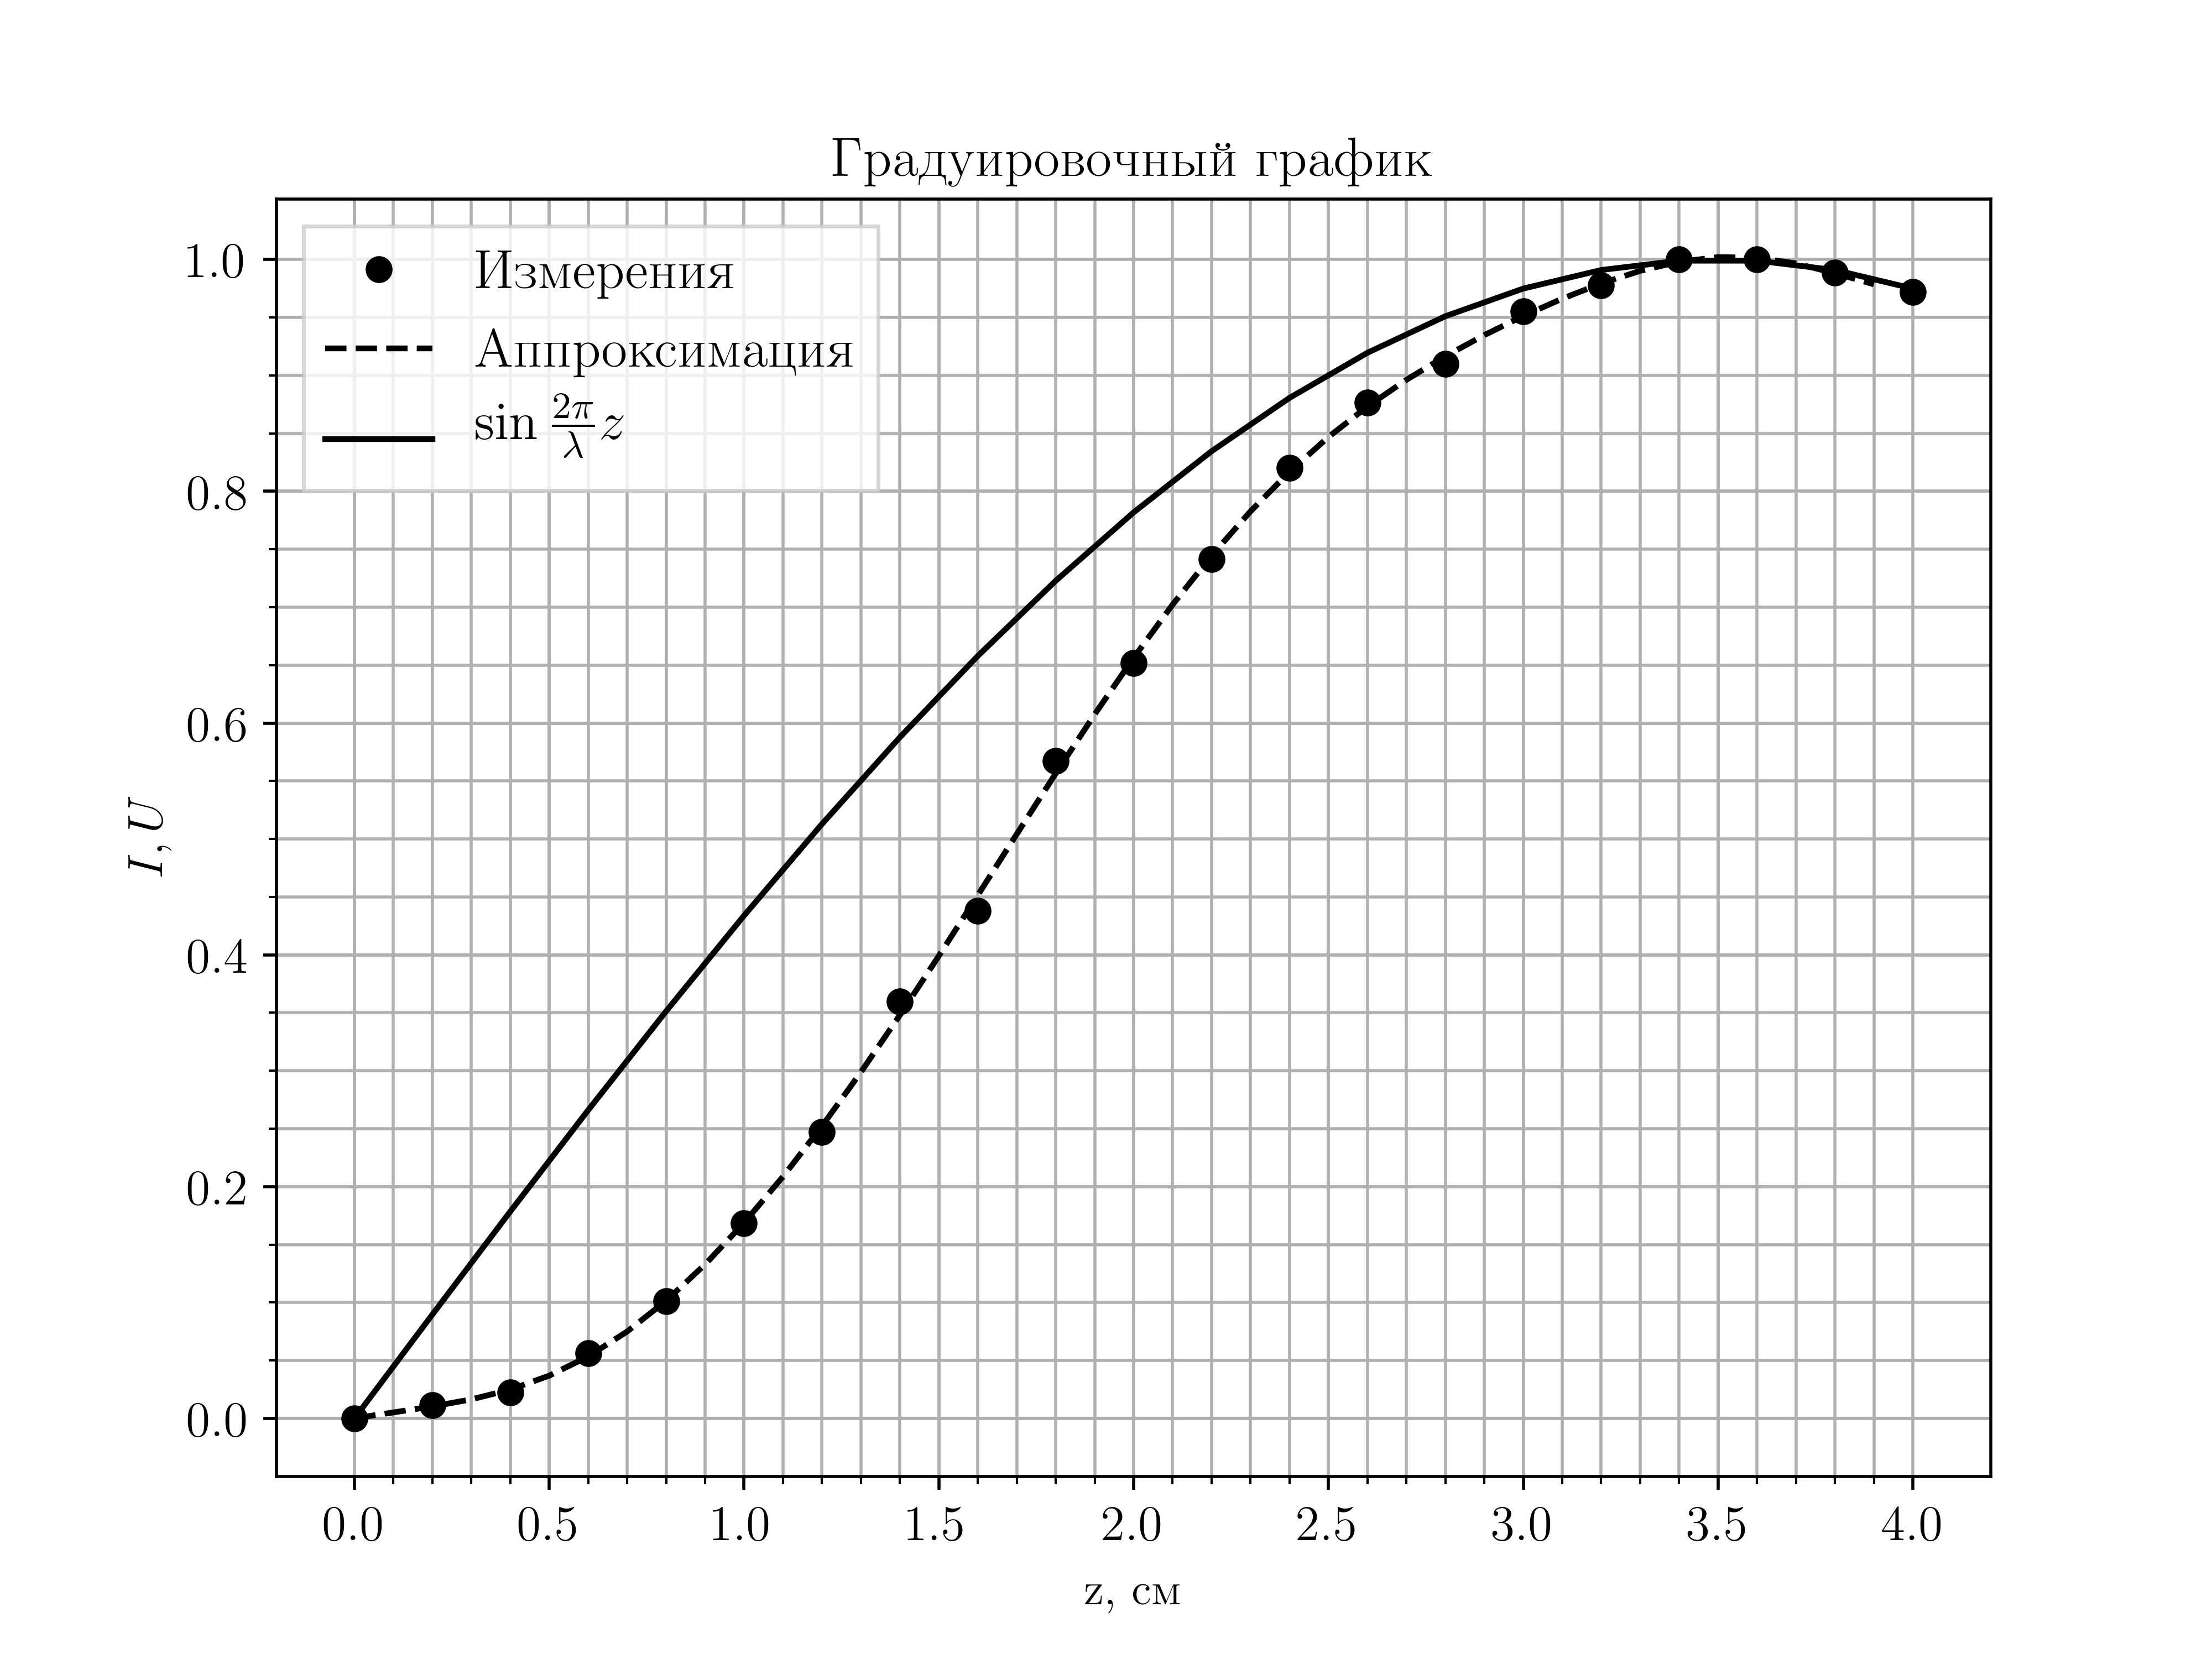
\includegraphics[width = 0.8\linewidth]{graphs/grad.png}
    \label{fig:2}
    \caption{}
\end{figure}

\textbf{Формула расчета импеданса нагрузки:}
\begin{equation}
    Z_H = Z_B\frac{i+K~tg(\frac{2 \pi }{\lambda_B} \Delta z_{min})}{iK+tg(\frac{2 \pi }{\lambda_B} \Delta z_{min})}
    \label{eq:21}
\end{equation}

\textbf{Формула расчета коэффициента отражения:}
\begin{equation}
    \Gamma = \frac{Z(z)-Z_B}{Z(z)+Z_B}
    \label{eq:22}
\end{equation}

В основном, работа производилась при частоте генератора $f = 2$ ГГц.
\subsection{Задание 1}
Определение координаты условного конца.

К волноводу подключается закорачивающий элемент, после чего с помощью измерительного прибора находится положение, в
котором показания минимальны (соответствует узлу стоячей волны):
$$ z^0_{min} = \frac{24.3+23.3}{2} = 23.8~cm $$

\subsection{Задание 2}
Определение длины волны в волноводе.

Измерение минимального расстояния между двумя узлами стоячй волны. Это расстояние соответствует половине длине волны
$\lambda_B$: $$ \lambda_B  = 15.1~cm $$

\subsection{Задание 3}
Измерение импеданса эталонов (коаксиальной линии с внутренним радиусом $a = 4~mm$, и внешним $b=17~mm$).
$$\textbf{КСВ}: K = \frac{U_{max}}{U_{min}}$$
\begin{table}[H]
    \centering
    \begin{tabular}{l|l|l|l|l|l|l|l}
       Тип нагрузки  & $z^0_{min}$, см & $\Delta z_{min}$, см & $I_{min}$ & $I_{max}$ & K &  $Z_H$ & $\Gamma$ \\ \hline
       Свободный &   23.8   &   6.25    &   4 ($\rightarrow 0$)  &   160   &  $\infty$ &   28.87$i$ &  \\ \hline
       Замкнутый &   23.8   &   3    &   2 ($\rightarrow 0$)   &   168   &  $\infty$  &  -153.89$i$  & -0.97  
    \end{tabular}
\end{table}

Теоретический расчет входного импеданса эталона:

Волновой импеданс коаксиальной линии($\varepsilon \simeq 1$):
\begin{equation}
    Z^0_{BX} = \frac{138}{\sqrt{\varepsilon}} ~lg(b/a) \simeq 86   
\end{equation}
$b,a$ - внутренний и внешний радиус линии. 

Свободного:
\begin{equation}
    Z_{BX}= -i Z^0_B~ctg~hl  \simeq 49.65i  
\end{equation}

Закороченного:
\begin{equation}
    Z_{BX}= i Z^0_B~tg~hl    \simeq -148.96i
\end{equation}

Таким образом, погрешность определения составила для закороченного конца :$\Delta Z \simeq 3 \% $, а для свободного:
$\Delta Z \simeq \textcolor{red}{41 \%}$

\subsection{Задание 4}
Измерение импеданса эталонов (коаксиальной линии), заполненных диэлектриком.

\begin{table}[H]
    \centering
    \begin{tabular}{l|l|l|l|l|l|l|l}
       Тип нагрузки  & $z^0_{min}$, см & $\Delta z_{min}$, см & $I_{min}$ & $I_{max}$ & K &  $Z_H$  & $\Gamma$\\ \hline
    Свободный &   23.8   &   3.5    &   4 ($\rightarrow 0$)  &   162   &  $\infty$ &  -475.7$i$ & \\ \hline
    Замкнутый &   23.8   &   0.3    &   5 ($\rightarrow 0$)   &   136   &  $\infty$    &  -6.3$i$ & -0.97 
    \end{tabular}
\end{table}

\subsection{Задание 5}
Измерение импеданса активного сопротивления ( $ R = 47 $ Ом ).

\begin{table}[H]
    \centering
    \begin{tabular}{l|l|l|l|l|l|l|l}
       Тип нагрузки  & $z^0_{min}$, см & $\Delta z_{min}$, см & $I_{min}$ & $I_{max}$ & K &  $Z_H$ &  \\ \hline
    Активное сопротивление &   23.8   &   1.9    &   10  &   80   &  2.4 & 35.7-36.1$i$ & 0.008 \\ 
    \end{tabular}
\end{table}

Так как величина активного сопротивления соответсвует согласованной нагрузке, то, как и ожидалось, $\Gamma \simeq 0.$
Чтобы оценить индуктивность подводящих проводов, надо записать импеданс нагрузки в виде, как если бы рассматривалось не только
активное сопротивление, но и индуктивность($ \omega = 2 \pi f $):
\begin{equation}
    Z_H = R + i\omega L =  35.7-36.1i
\end{equation}

\subsection{Задание 6}
Измерение импеданса конденсатора, нахождение собственной частоты колебательного контура.

\begin{table}[H]
    \centering
    \begin{tabular}{l|l|l|l|l|l|l|l}
       $f$,ГГц  & $z^0_{min}$, см & $\Delta z_{min}$, см & $I_{min}$ & $I_{max}$ & K &  $Z_H$ & $\Gamma$  \\ \hline
    2 &   23.8   &   5.9    &   2 ($\rightarrow 0$)  &   155   &   &  &  \\ \hline
    2.015 &   16.45   &   -1.75    &   2 ($\rightarrow 0$)   &   35   &     &   & 
    \end{tabular}
\end{table}

\subsection{Вывод}




\end{document}